\lecture{21}{8 maggio 2024}
\subsection{Formule di Fresnel}
Oggi studiamo la relazione fra polarizzazione e passaggio fra due mezzi ottici distinti. Supponiamo che la polarizzazione non cambi al passaggio fra due mezzi e nella riflessione (trascuriamo materiali con molecole chirali e altre stranezze).
\begin{figure}[H]
	\centering
	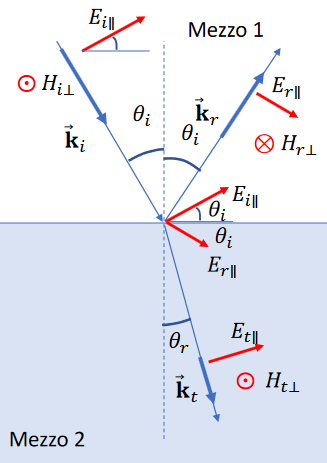
\includegraphics[width=0.4\textwidth]{screenshots/2024-05-08-09-15-56.png}
\end{figure}
Se l'incidenza dell'onda non è normale, allora nello spazio esiste un piano definito dalla normale alla superficie e dalla direzione di moto dell'onda. La componente del campo elettrico che sta su questo piano ha proprietà di riflessione e rifrazione diverse da quelle della componente normale a tale piano (per ora studiamo la componente del campo elettrico parallela al piano d'incidenza e insieme la componente perpendicolare del campo magnetico). I versi in figura sono stati messi coerentemente con quanto fatto ieri per \(\theta _i \to 0\), sia per il campo elettrico che per il campo magnetico (N.B.: queste sono tutte scelte arbitrarie!).
Le considerazioni fatte ieri sulla circuitazione valgono anche in questo caso:
\begin{equation}
	E_{i \parallel} \cos (\theta _i) + E_{r \parallel} \cos (\theta _i) = E_{t \parallel} \cos (\theta _r)
\end{equation}
Il campo magnetico invece è perpendicolare al piano incidente e parallelo alla superficie di separazione, quindi ho la relazione già studiata:
\begin{equation}
	H_{i \perp } - H_{r \perp } = H_{t \perp } \implies n1 E_{i \parallel} - n_1 E_{r \parallel} = n_2 E_{t \parallel}
\end{equation}
Pongo
\begin{align}
	\alpha &= \frac{\cos (\theta _r)}{\cos (\theta _i)} &
	\beta &= \frac{n_2}{n_1}
\end{align}
da cui si ha
\begin{equation}
	\begin{cases}
		E_{i \parallel} + E_{r \parallel} = \alpha E_{t \parallel}\\
		E_{i \parallel} - E_{r \parallel} = \beta E_{t \parallel}	
	\end{cases}
\end{equation}
Si ottengono così le formule di Fresnel per il campo elettrico parallelo:
\begin{figure}[H]
	\centering
	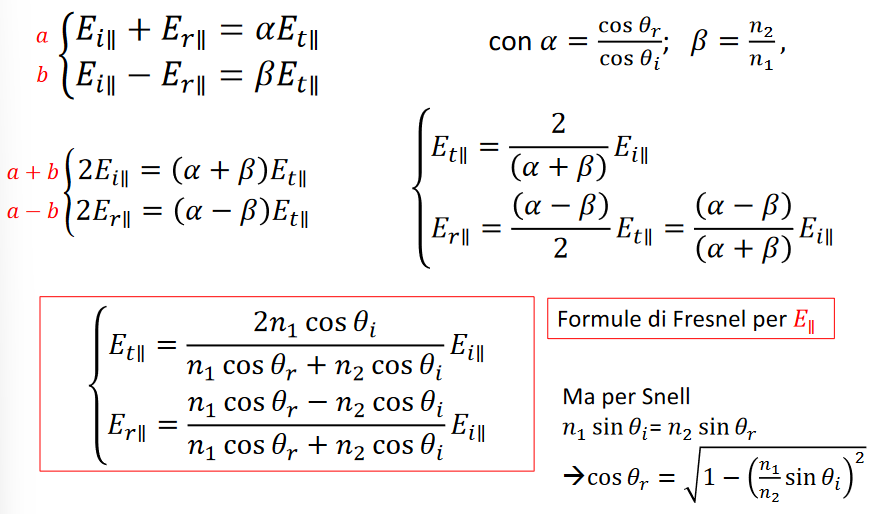
\includegraphics[width=0.5\textwidth]{screenshots/2024-05-08-09-32-20.png}
\end{figure}
Disegniamo quello che sta accadendo:
\begin{figure}[H]
	\centering
	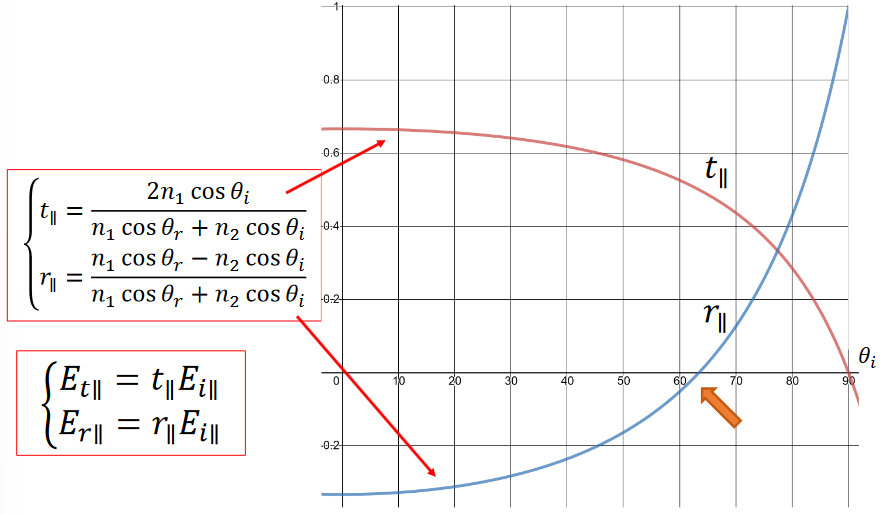
\includegraphics[width=0.5\textwidth]{screenshots/2024-05-08-09-33-56.png}
\end{figure}
Sapendo che \(I= \quotient{1}{Z} \langle E ^{2}  \rangle \) e ponendo \(R_\parallel = r_\parallel ^{2} \), si ottiene immediatamente che \(I_{r \parallel} = R_\parallel I_{i \parallel}\). Posto invece \(T_\parallel = \frac{4 \alpha \beta }{(\alpha + \beta )^{2} }\), si ha \(I_{t \parallel} = T_\parallel I_{i \parallel} \quotient{\cos (\theta _i)}{\cos (\theta _r)} \).
\begin{figure}[H]
	\centering
	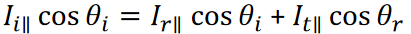
\includegraphics[width=0.4\textwidth]{screenshots/2024-05-08-09-38-56.png}
\end{figure}
Non si conserva l'intensità. Per fortuna la fisica è salva, perché l'importante è che si conservi l'energia. L'intensità non si conserva perché varia la superficie su cui è distribuita la potenza dell'onda.

Studiamo ora il caso del campo elettrico perpendicolare al piano d'incidenza e il campo magnetico parallelo al piano d'incidenza.
\begin{figure}[H]
	\centering
	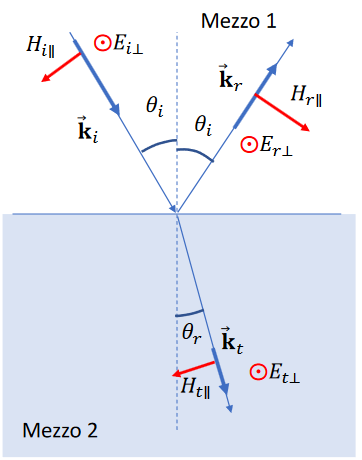
\includegraphics[width=0.4\textwidth]{screenshots/2024-05-08-09-40-42.png}
\end{figure}
Per la continuità del campo elettrico usiamo la formula dell'incidenza normale: \(E_{i \perp } + E_{r \perp } = E_{t\perp } \). Per il campo magnetico invece vale un ragionamento analogo a prima, da cui si ottiene \(H_{i\parallel }\cos (\theta _i) - H_{r\parallel } \cos (\theta _i) = H_{t\parallel } \cos (\theta _r)   \). Pongo \(\alpha, \beta \) come prima e trovo
\begin{figure}[H]
	\centering
	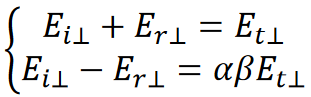
\includegraphics[width=0.2\textwidth]{screenshots/2024-05-08-09-44-26.png}
\end{figure}
Svolgendo nuovamente i calcoli come prima troviamo le formule di Fresnel per il campo elettrico perpendicolare:
\begin{figure}[H]
	\centering
	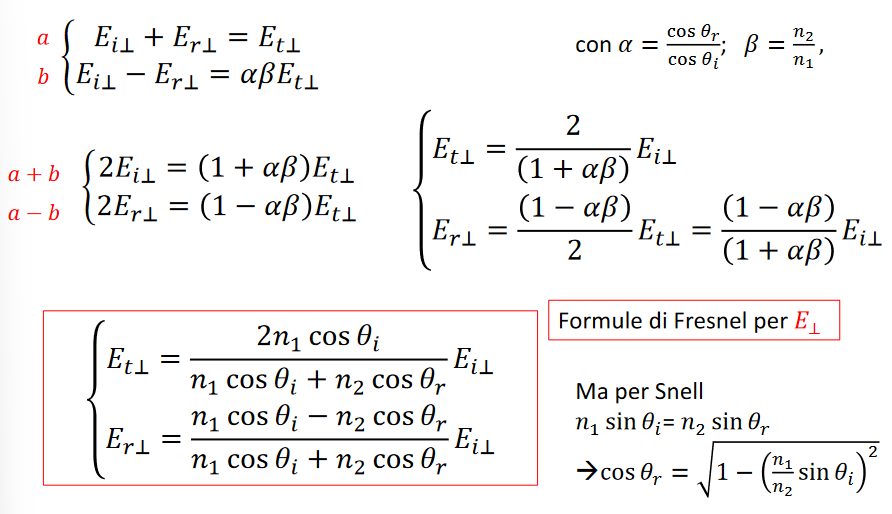
\includegraphics[width=0.5\textwidth]{screenshots/2024-05-08-09-45-58.png}
\end{figure}
Disegniamo quello che sta succedendo:
\begin{figure}[H]
	\centering
	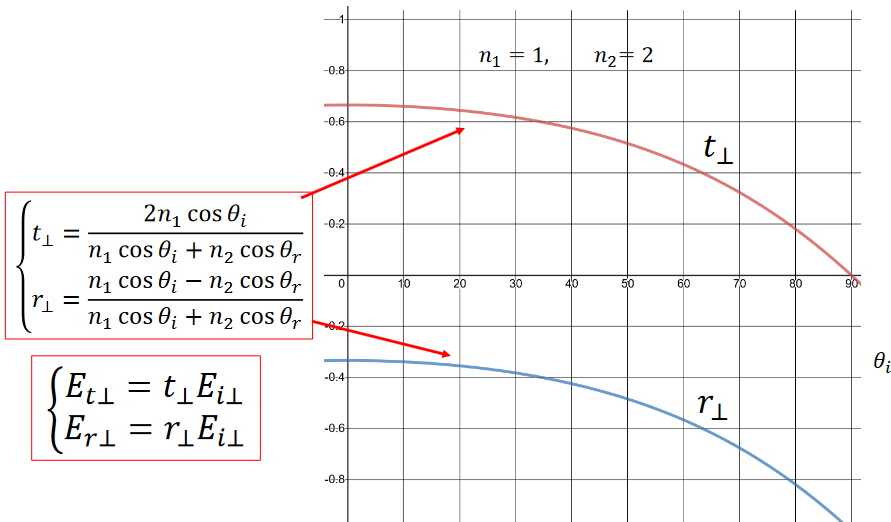
\includegraphics[width=0.5\textwidth]{screenshots/2024-05-08-09-47-02.png}
\end{figure}
Anche sull'intensità facciamo lo stesso identico calcolo di prima. Chiamiamo \(R_{\perp } = r_{\perp }^{2}   \) e \(T_{\perp } = \frac{4 \alpha \beta }{(1 + \alpha \beta )^{2} } \). Si ha che \(I_{r\perp } = R_{\perp }I_{i\perp }   \) e \(I_{t\perp }= T_{\perp }I_{i\perp } \frac{\cos (\theta _i)}{\cos (\theta_r)}  \), per cui risulta:
\begin{figure}[H]
	\centering
	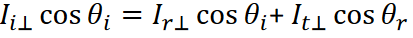
\includegraphics[width=0.3\textwidth]{screenshots/2024-05-08-09-50-30.png}
\end{figure}
Stesso discorso di prima sull'energia.

Caso per caso devo capire quale è la componente perpendicolare e quale la componente parallela dell'onda incidente.

\paragraph{Angolo di Brewster}
% TODO: recupera tutto questo discorso da slide
Abbiamo visto che c'è un angolo per cui \(r_{\parallel } =0	\). Questo equivale a dire che \(n_1 \cos (\theta _r) = n_2 \cos (\theta _i)\). Dalla legge di Snell, questa relazione è verificata quando \(\theta _i + \theta _r = \frac{\pi}{2}\). In questo caso \(\theta _i = \theta _B\) "angolo di Brewster". La luce riflessa è totalmente polarizzata.
\begin{formula}
	[Angolo di Brewster]
	Dall'equazione che definisce l'angolo di Brewster e dalla legge di Snell si ricava che:
	\begin{equation}
		\tan (\theta _B) = \frac{n_2}{n_1}
	\end{equation}
\end{formula}

\section{Interferenza}
Questo argomento è particolarmente importante perché ci permette di capire che cosa sia la luce. C'erano due grandi gruppi: i sostenitori della teoria corpuscolare e quelli della teoria ondulatoria. L'idea di Young era che se la luce è un'onda allora deve mostrare i comportamenti tipici delle onde, che non possono essere spiegati dalla teoria corpuscolare: diffrazione e interferenza.
\begin{figure}[H]
	\centering
	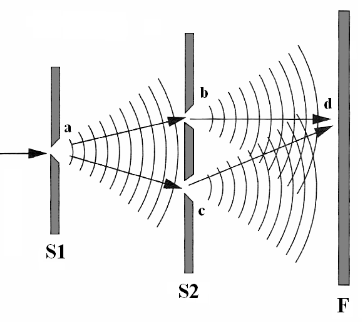
\includegraphics[width=0.3\textwidth]{screenshots/2024-05-08-10-19-39.png}
\end{figure}
Viene prodotta luce monocromatica, diffusa attraverso lo schermo S1 e poi divisa in due sorgenti secondarie coerenti dallo schermo S2. Il risultato osservato sono delle figure di interferenza sullo schermo di osservazione F. Sembra che gli ondulatori avessero ragione (plot twist nel 1900). La stessa cosa succede anche con gli elettroni e anche mandando un fotone alla volta. La meccanica quantistica spiega questo comportamento. Rimaniamo coi piedi per terra e studiamo l'interferenza alla Young.
\begin{figure}[H]
	\centering
	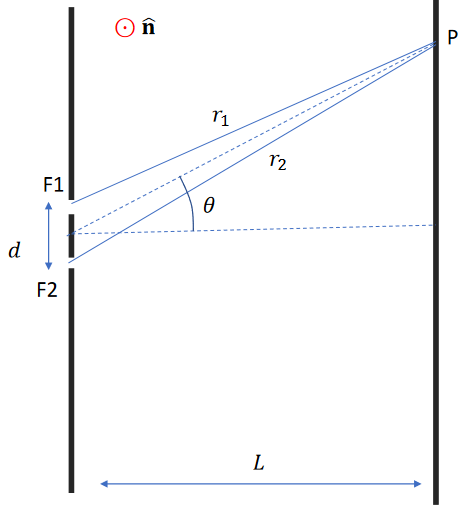
\includegraphics[width=0.4\textwidth]{screenshots/2024-05-08-10-27-22.png}
\end{figure}
I campi in uscita dalle fenditure sono \(\vec{E}_1 (F1) = E_0 e^{-i \omega t} \vec{\hat{n}}\) e \(\vec{E}_2(F2) = E_0 e^{i \omega t} \vec{\hat{n}}\), mentre in P sono \(\vec{E}_1 (P) = E_0^{\prime} e^{i(kr_1 - \omega t)} \vec{\hat{n}}\) e \(\vec{E}_2 (P) = E_0^{\prime} e^{i (kr_2 - \omega t)} \vec{\hat{n}}\). Per semplicità ipotizziamo che gli angoli siano piccoli e che quindi siano uguali le ampiezze (vanno come \(\quotient{1}{r} \)).
\begin{figure}[H]
	\centering
	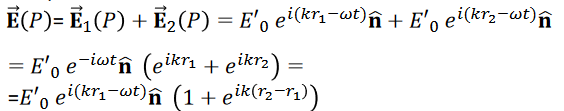
\includegraphics[width=0.4\textwidth]{screenshots/2024-05-08-10-31-11.png}
\end{figure}
Per angoli piccoli posso approssimare \(r_2 - r_1 = d \sin (\theta )\). Lo sfasamento fra i due raggi è \(\Delta \varphi = k (r_2 - r_1) = kd \sin (\theta )\). Questo vale se lo schermo è molto lontano e se gli angoli sono piccoli. Si hanno due casi estremi:
\begin{description}
	\item[Interferenza costruttiva] Si ha campo massimo se \(\Delta \varphi = 2n \pi\), da cui \(\sin (\theta ) = \frac{n \lambda }{d} \) con \(n=0, \pm 1, \pm 2, \dots , \pm \infty \). Il campo è doppio e l'intensità quadruplica.
	\item[Interferenza distruttiva] Si ha campo minimo per \(\Delta \varphi = (2n + 1) \pi \implies \sin (\theta ) = (n + \frac{1}{2}) \frac{\lambda }{d}\). Il campo è nullo e l'intensità anche.
\end{description}
Per l'intensità in generale si ritrova la formula dell'interferenza delle onde sonore:
\begin{figure}[H]
	\centering
	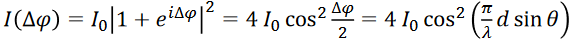
\includegraphics[width=0.4\textwidth]{screenshots/2024-05-08-10-39-46.png}
\end{figure}
Osserviamo che \(\langle I(\Delta \varphi ) \rangle = 2 I_0\), quindi l'intensità si conserva. Però l'energia appare redistribuirsi sullo schermo, solo con zone di accumulo e zone di perdita.

\paragraph{Fattore di controllo}
Ciò che controlla l'effetto dell'interferenza è il rapporto \(\quotient{d}{\lambda } \). Per \(d\ll \lambda \) sullo schermo si ha un solo massimo di interferenza, si ha una diffusione della luce. Per \(d \gg \lambda \) non ho più sorgenti puntiformi F1 ed F2, i raggi non sono più colineari e quindi i calcoli fatti non valgono. Si possono avere problemi di coerenza e non si vede più la figura d'interferenza. Per \(d>\lambda \) ma \(d\) piccolo vale l'approssimazione delle sorgenti puntiformi F1 ed F2 e si riesce a osservare il fenomeno di interferenza.

\subsection{Interferenza con più sorgenti}
\begin{figure}[H]
	\centering
	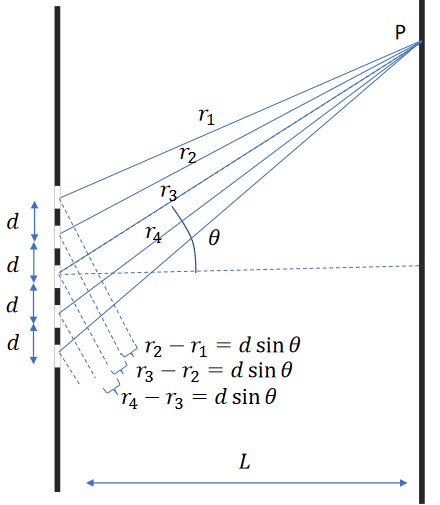
\includegraphics[width=0.4\textwidth]{screenshots/2024-05-08-10-46-30.png}
\end{figure}
Consideriamo un sistema con N sorgenti monocromatiche, coerenti ed uguali, distribuite a distanze fisse su uno schermo. Il campo in P è dato da
\begin{figure}[H]
	\centering
	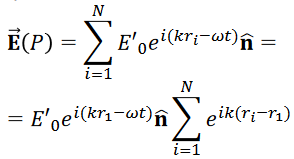
\includegraphics[width=0.2\textwidth]{screenshots/2024-05-08-10-47-17.png}
\end{figure}
Opero la stessa approssimazione di prima: piccoli angoli, quindi \(r_m = r_{m-1} = d \sin (\theta )\) e in P considero uguali le N ampiezze. Pongo \(\varphi = kd \sin (\theta )\) e ottengo che
\begin{equation}
	\sum_{i=1}^{N} e^{i k(r_i - r_1)} = 1 + e^{i \varphi } + e^{i 2 \varphi } + \cdots + e^{(N-1) i \varphi }
\end{equation}
È un pezzo di serie geometrica, quindi
\begin{figure}[H]
	\centering
	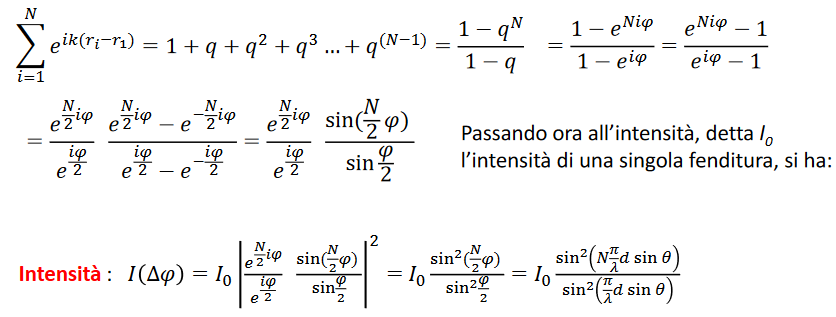
\includegraphics[width=0.4\textwidth]{screenshots/2024-05-08-10-53-48.png}
\end{figure}
Se \(N=5\), \(I_{max} = 25 I_0 \). Se \(N=10\), \(I_{max}=100 I_0 \). Si osservano dei minimi e massimi, con massimi principali di intensità proporzionale a \(N^{2} \) e massimi e secondari. I minimi sono sempre ad intensità nulla e quasi equispaziati. La larghezza dei massimi principali dipende da \(N\).
\begin{figure}[H]
	\centering
	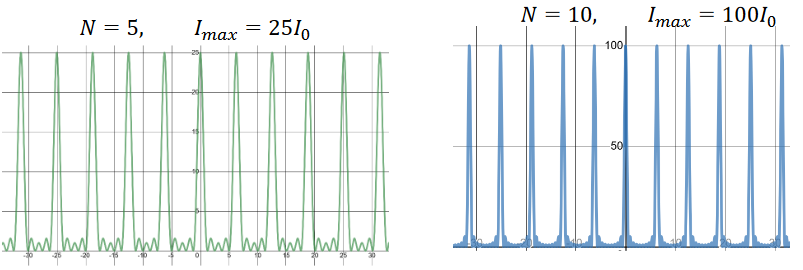
\includegraphics[width=0.5\textwidth]{screenshots/2024-05-08-10-57-48.png}
\end{figure}
Si hanno minimi per \(N \frac{\pi}{\lambda } d \sin (\theta ) = n \pi\), cioè per \(\sin (\theta ) = \frac{n \lambda }{Nd}\) con \(n= \pm 1, \pm 2, \dots, \infty \) tranne quando \(n=0, \pm N, \pm 2N, \dots \). In tali casi infatti il denominatore vale 0 e la formula per l'intensità ha espressione indeterminata. Lo studio del limite porta a verificare che in questi casi si hanno massimi principali, ossia quando \(\frac{\pi}{\lambda } d \sin (\theta )= m \pi \) (come per l'interferenza con due fenditure!).
Nell'ipotesi di piccoli angoli possiamo stimare la larghezza a metà altezza del picco come
\begin{figure}[H]
	\centering
	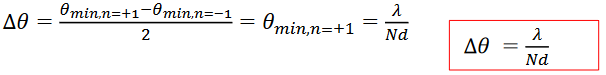
\includegraphics[width=0.4\textwidth]{screenshots/2024-05-08-11-02-12.png}
\end{figure}